
\subsection{LRU}
\label{sec:algorithms:lru}

\begin{figure}[ht]
    \centering
    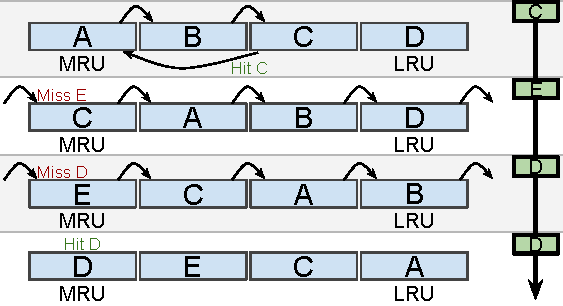
\includegraphics[width=.65\textwidth]{figures/algorithms/LRU}
    \caption{LRU managed 4-way cache set.}
    \label{fig:algorithms:lru_example}
\end{figure}

\noindent
Least recently used (LRU) replacement, or some simplification of LRU, is one of the dominant cache management algorithms in hardware today. 
As a result, LRU is normally used as the baseline for comparisons when presenting new cache management algorithms~\cite{Jaleel2010,Qureshi2006,Qureshi2007}.

The LRU algorithm relies on the temporal locality of data accesses; it assumes that recently accessed data has a higher reuse frequency than less recently accessed data.
Theoretically one can envision a cache set managed by LRU as a stack, where recently accessed cache blocks are near the top and less recently accessed blocks are near the bottom.
The bottom position of the stack is the LRU position, and the top position is the most recently used (MRU) position.
In a hardware implementation, the blocks are not stored in a sorted fashion, but additional storage bits are used to keep track of LRU positions.
The replacement policy of LRU is to evict the least recently used cache block, the one on the bottom of the LRU stack.
The insertion and promotion policy of LRU is the same; a inserted or accessed block is always moved to the MRU position unless it is already there.

Figure~\ref{fig:algorithms:lru_example} shows how a 4-way cache set managed by LRU replacement handles three requests. 
Initially, the set contains four blocks; A, B, C and D. 
A is in the MRU position while D is in the LRU position.
The first request is for block C; this is a hit, and that causes the block to move to the MRU position, pushing both block A and B one step closer to the LRU position.
The second request is made to block E; this block is not present in the cache.
The LRU algorithm evicts block D at the LRU position and then places block E at the MRU position.
Finally, another request is made to block E. Nothing changes since the block already is at the MRU position.

One important result of the LRU insertion, promotion, and replacement policies is that an LRU managed cache satisfies the \textit{stack property}.
Given a 4-way LRU managed cache with counters that count the number of hits in each way; then we know that the number of misses in a 3-way LRU managed cache equals the misses in the 4-way cache plus the number of hits in the 4th cache way.
This effect occurs because any request that hits in the 4th way of the 4-way cache would miss in the 3-way cache, but in both caches the requested block is then moved to the MRU position.
No blocks can enter the cache set at any other position than the MRU.
As a result, the state of the three first ways of the caches is always identical given an identical memory request sequence.
The same argument holds for a 2-way cache, by summing the hits in the third and fourth way of the 4-way cache we get the additional misses in a 2-way cache.
This property generalizes; we can find the relative miss rate of any LRU managed cache with $1$ to $n$ ways by having a single n-way cache with access counters per way.
If we additionally have a total miss counter in the n-way cache we can also find the absolute number of misses for each cache size.

LRU is a simple replacement algorithm that is usable in both private and shared caches.
In shared caches, LRU will favor access frequency, giving cores that issue many cache requests more cache space than those who issue fewer requests. 
In some cases, this might be an acceptable solution. 
However, as we will discover, several thread-aware replacement algorithms claiming to outperform LRU exists. 
